\documentclass{beamer}

\usepackage[utf8]{inputenc}
\usepackage{tikz}
%\usetikzlibrary{decorations.pathreplacing,calc}
%\newcommand{\tikzmark}[1]{\tikz[overlay,remember picture] \node (#1) {};}
\usepackage{graphicx}
\usepackage{picture}
\usepackage{listings}
\author{Jonathan Boidol, Rene Schoeffel, Yann Sp\"ori}
\title{HyPnOBrain}
\subtitle{your homology based HPO neural network predictor}
\date{January 23, 2014 }
%\usepackage{default}



\begin{document}

{
\usebackgroundtemplate%
{%
   % 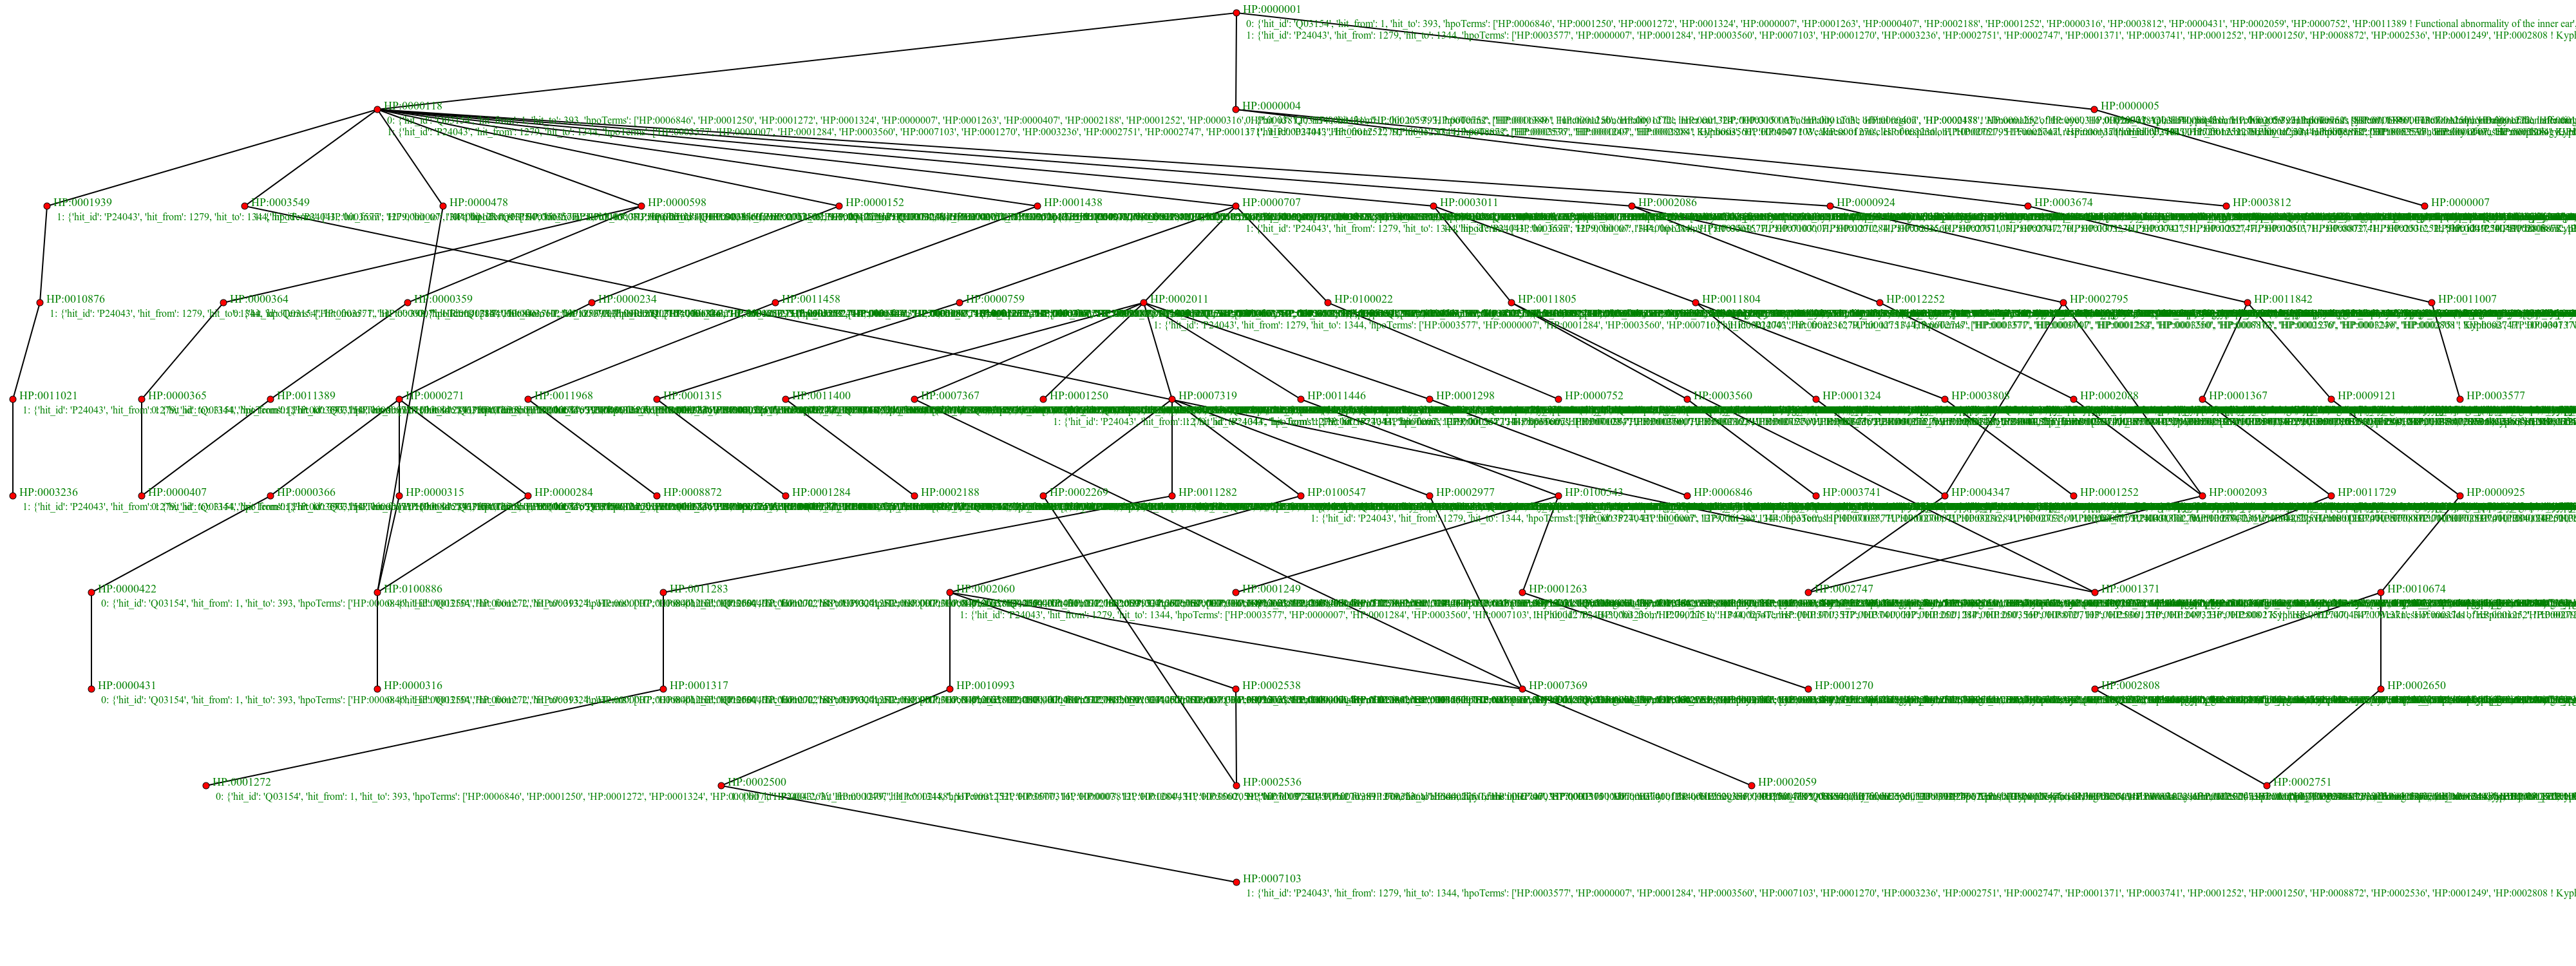
\includegraphics[width=\paperwidth,height=\paperheight]{Q03154.png}%
    \vbox to \paperheight{\vfil\hbox to \paperwidth{\hfil\tikz\node[opacity=0.3] {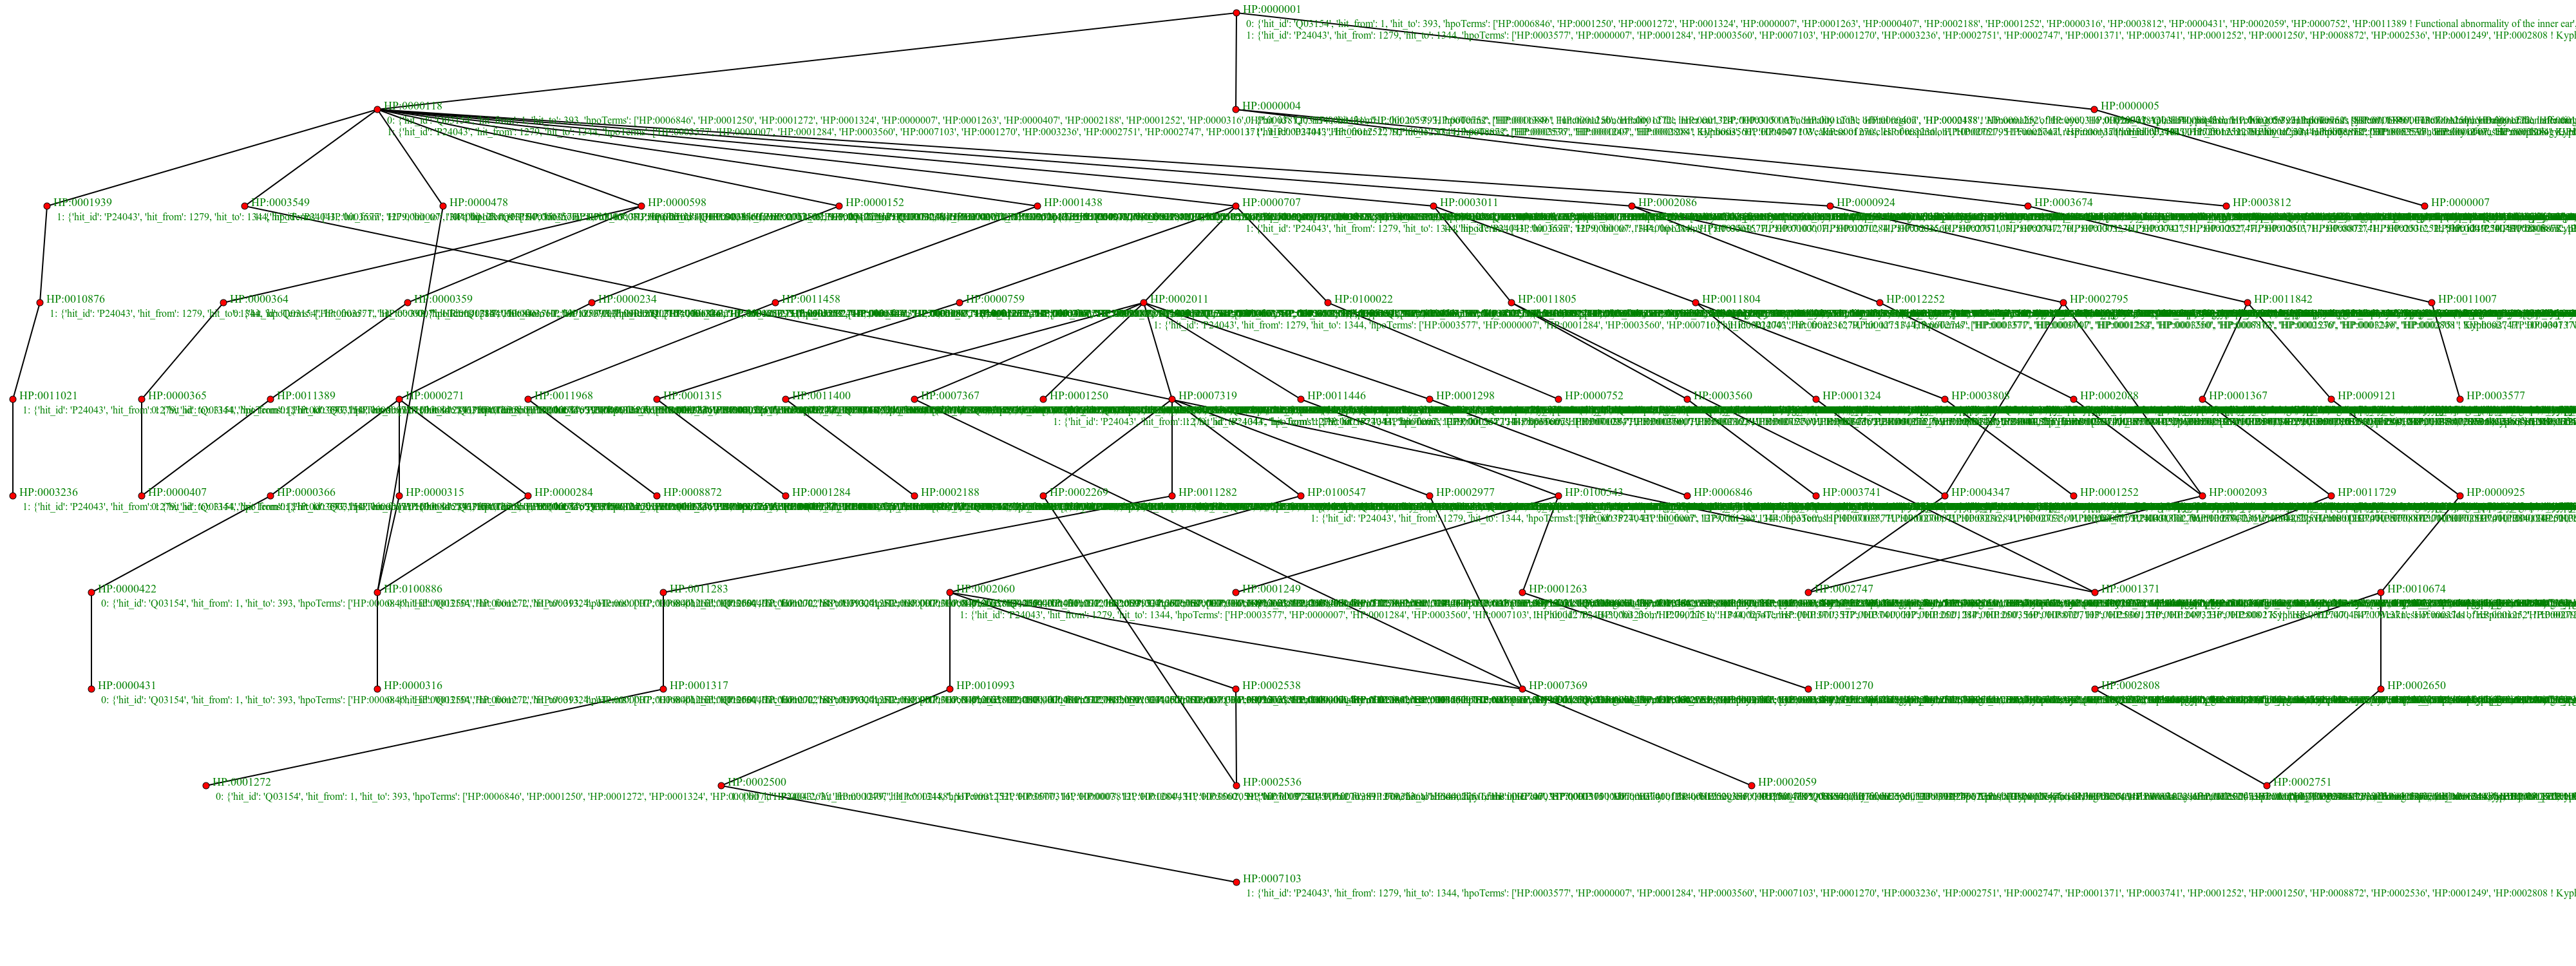
\includegraphics[scale=0.11]{Q03154.png}};\hfil}\vfil}
    
}
 
\begin{frame}
\maketitle
 
\end{frame}
}
\begin{frame}
  \frametitle{Homology based function prediction}
  General approach:
  \begin{itemize}
  	\item Search for annotated similar sequences (hits) and transfer annotations
  	\item HPO is hierarchical: Merge found annotations from different hits
  	\item Calculate confidence for every annotation from some distance measure to the hits
  \end{itemize}
  \hfill\\  \hfill\\  \hfill\\
  \hfill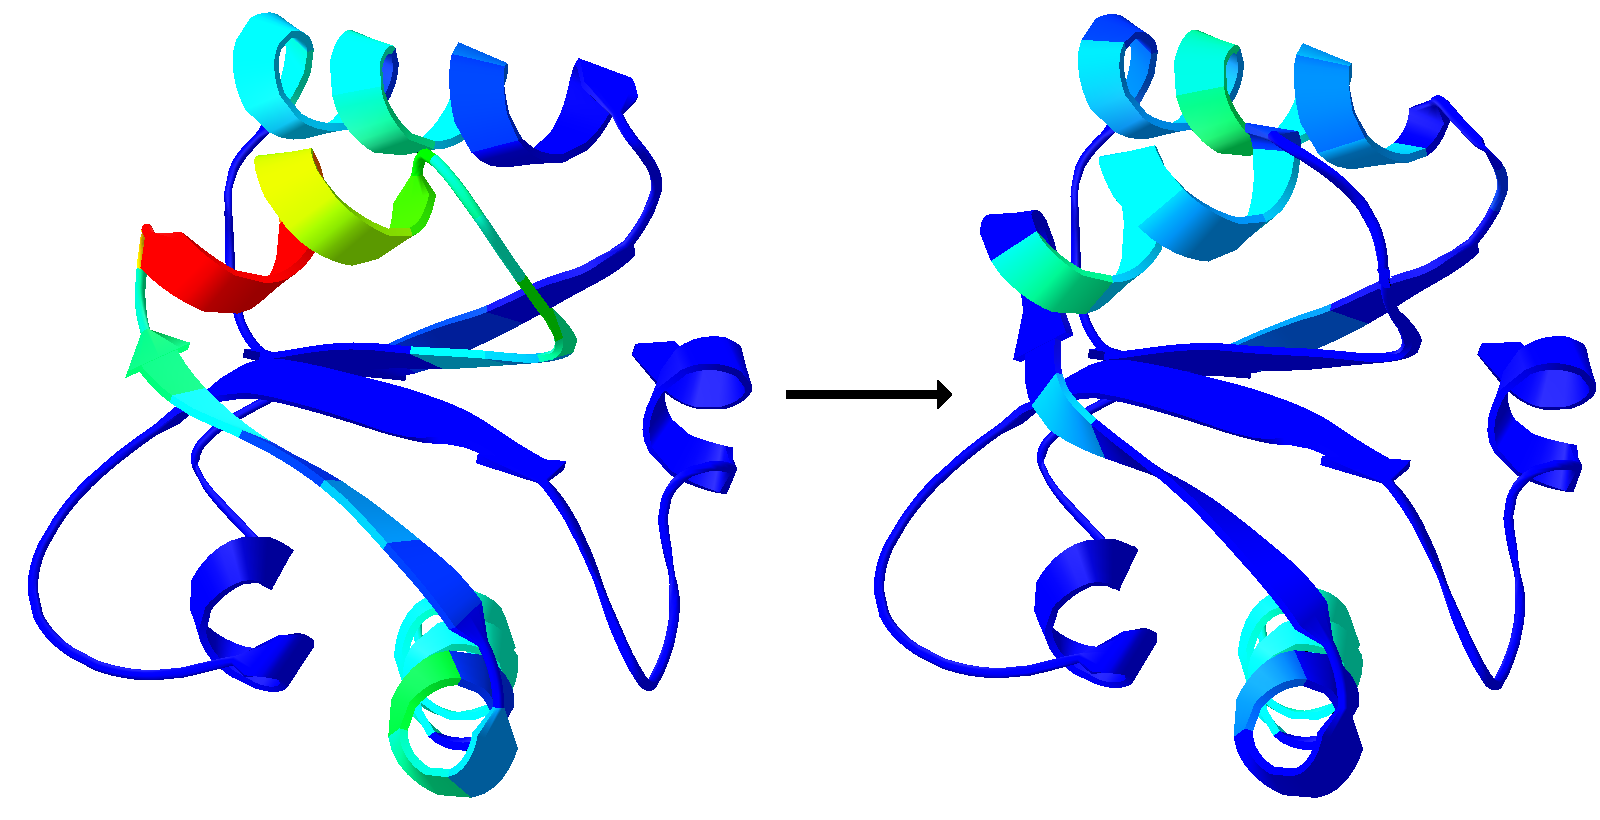
\includegraphics[width=0.4\textwidth]{homologs.png}

\end{frame}

\begin{frame}
	\frametitle{Preparations and Predictor input}
		\begin{itemize}
			\item Prepare databases for annotated sequences
			\item Represent HPO Graph in predictor
			\item Merge trees corresponding to hits
		\end{itemize}
		\begin{minipage}{0.2\textwidth}
			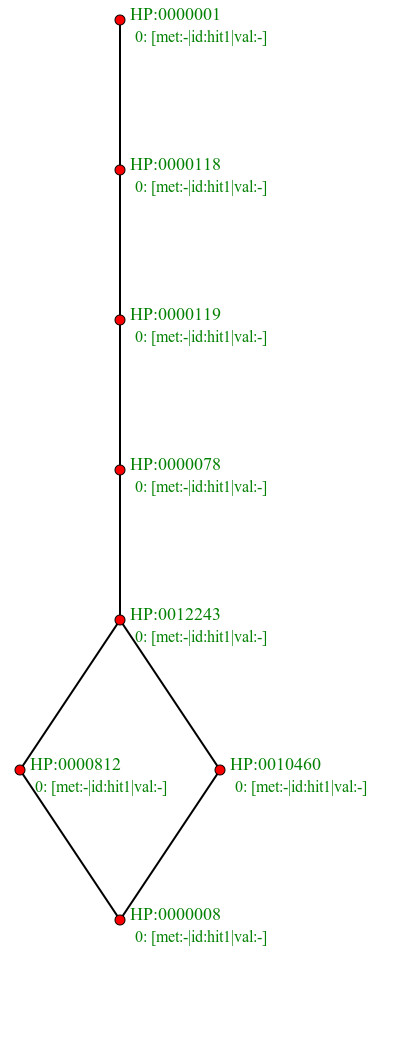
\includegraphics[width=\textwidth]{p1.jpg}	
		\end{minipage}$+$\hspace*{1em}
		\begin{minipage}{0.1\textwidth}
			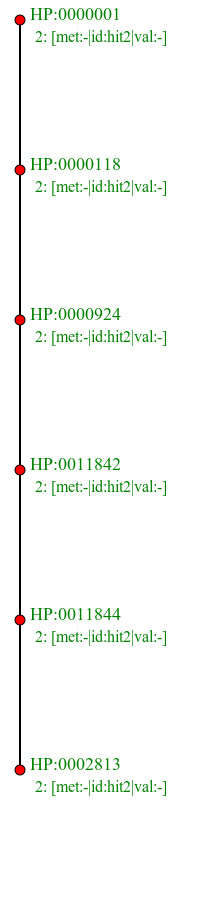
\includegraphics[width=\textwidth]{p2.jpg}\\
			\vspace*{1.0em}
		\end{minipage}$\Rightarrow$
		\begin{minipage}{0.3\textwidth}
		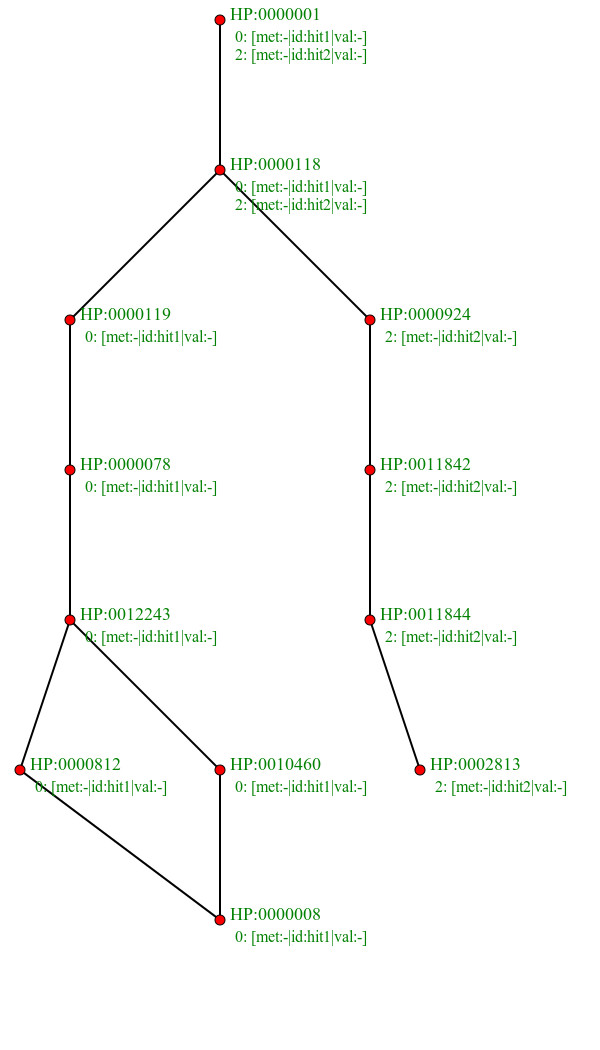
\includegraphics[width=\textwidth]{g.jpg}
		\end{minipage}
		
		
\end{frame}

\begin{frame}
	\frametitle{Derived features}
	\begin{itemize}
		\item each node is assigned 12 features derived from the merged tree
		\item[] \begin{itemize}
					\item length of query sequence 
					\item number of hits
					\item longest hit
					\item avg. hit	
					\item min. E-value	
					\item avg. E-value 
					\item product of E-values
					\item best E-value from blast or hhblits 
					\item min. height in HPO-tree
					\item max. height in HPO-tree
					\item max overlap of query and all hits
					\item length of best hit
					\makebox(0,0){\put(65,17\normalbaselineskip){%
               $\left.\rule{0pt}{6.1\normalbaselineskip}\right\}$ \,[3, 0.0074, 0.45, 4.2e-7, 84, $\dots$]}}
				\end{itemize}
				\item use neural network to calculate confidence per node 
	\end{itemize}
\end{frame}

\begin{frame}
	\frametitle{Final network architecture}
\begin{center}
	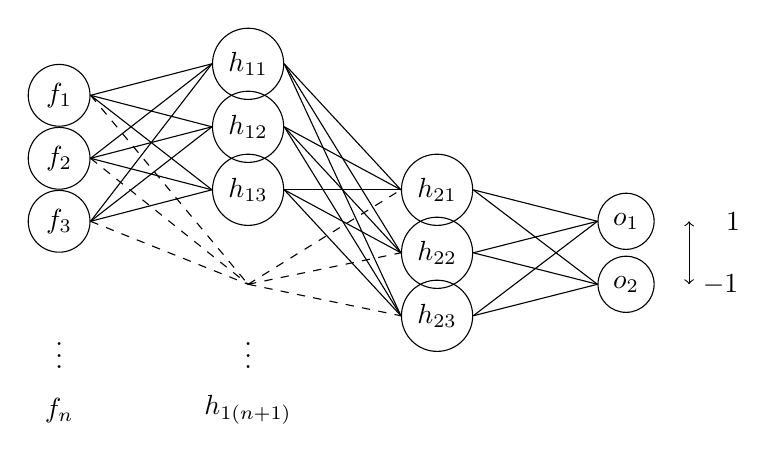
\begin{tikzpicture}[scale=0.8]
	
	%input nodes
	\node[draw, circle] (f1) at (0,4){$f_1$};
	\node[draw, circle] (f2) at (0,3){$f_2$};
	\node[draw, circle] (f3) at (0,2){$f_3$};
	\node[] at (0,0){$\vdots$};
	\node[] (fn) at (0,-1){$f_n$};
	
	%first hidden level
	\node[draw, circle] (h11) at (3,4.5){$h_{11}$};
	\node[draw, circle] (h12) at (3,3.5){$h_{12}$};
	\node[draw, circle] (h13) at (3,2.5){$h_{13}$};
	\node[] at (3,0){$\vdots$};
	\node[] (h1n) at (3,-1){$h_{1(n+1)}$};	
	
	%second hidden level
	\node[draw, circle] (h21) at (6,2.5){$h_{21}$};
	\node[draw, circle] (h22) at (6,1.5){$h_{22}$};
	\node[draw, circle] (h23) at (6,0.5){$h_{23}$};
	
	
	%output level
	\node[draw, circle] (o1) at (9,2){$o_{1}$};
	\node[draw, circle] (o2)at (9,1){$o_{2}$};
	
	\draw [<->](10,1) -- (10,2);
	\node[] (out1) at (10.7,2){$1$};
	\node[] (out2) at (10.5,1){$-1$};
	
	\draw (f1.east) -- (h11.west);
	\draw (f1.east) -- (h12.west);
	\draw (f1.east) -- (h13.west);
	\draw (f1.east)[dashed] -- (3,1);

	\draw (f2.east) -- (h11.west);
	\draw (f2.east) -- (h12.west);
	\draw (f2.east) -- (h13.west);
	\draw (f2.east)[dashed] -- (3,1);

	\draw (f3.east) -- (h11.west);
	\draw (f3.east) -- (h12.west);
	\draw (f3.east) -- (h13.west);
	\draw (f3.east)[dashed] -- (3,1);
	
	\draw (h11.east) -- (h21.west);
	\draw (h11.east) -- (h22.west);
	\draw (h11.east) -- (h23.west);

	\draw (h12.east) -- (h21.west);
	\draw (h12.east) -- (h22.west);
	\draw (h12.east) -- (h23.west);

	\draw (h13.east) -- (h21.west);
	\draw (h13.east) -- (h22.west);
	\draw (h13.east) -- (h23.west);

	\draw (3,1)[dashed] -- (h21.west);
	\draw (3,1)[dashed] -- (h22.west);
	\draw (3,1)[dashed] -- (h23.west);
	
	\draw (h21.east) -- (o1.west);
	\draw (h21.east) -- (o2.west);
	
	\draw (h22.east) -- (o1.west);
	\draw (h22.east) -- (o2.west);
	
	\draw (h23.east) -- (o1.west);
	\draw (h23.east) -- (o2.west);
	
	\end{tikzpicture}
\end{center}
	\hfill\\
	\begin{itemize}
		\item different architectures evaluated
		\item fully connected net with two hidden layers
		\item two output nodes trained for the two possible predictions
		\item difference of predictions as confidence
	\end{itemize}	
\end{frame}

\begin{frame}
	\frametitle{Validation}
	
	\begin{itemize}
		\item Inspection of the dataset shows: Most sequences have pairwise similarity $< 80\%$
		\item[] $\Rightarrow$ no significant bias in the dataset caused by very close homologs
		\item 10-fold crossvalidation over 2815 sequences 
		\item Calculate precision and recall per test sequence and average over all sequences
		\item Final model trained on all sequences
	\end{itemize}
\end{frame}

\begin{frame}
	\frametitle{Results}
	\begin{center}
	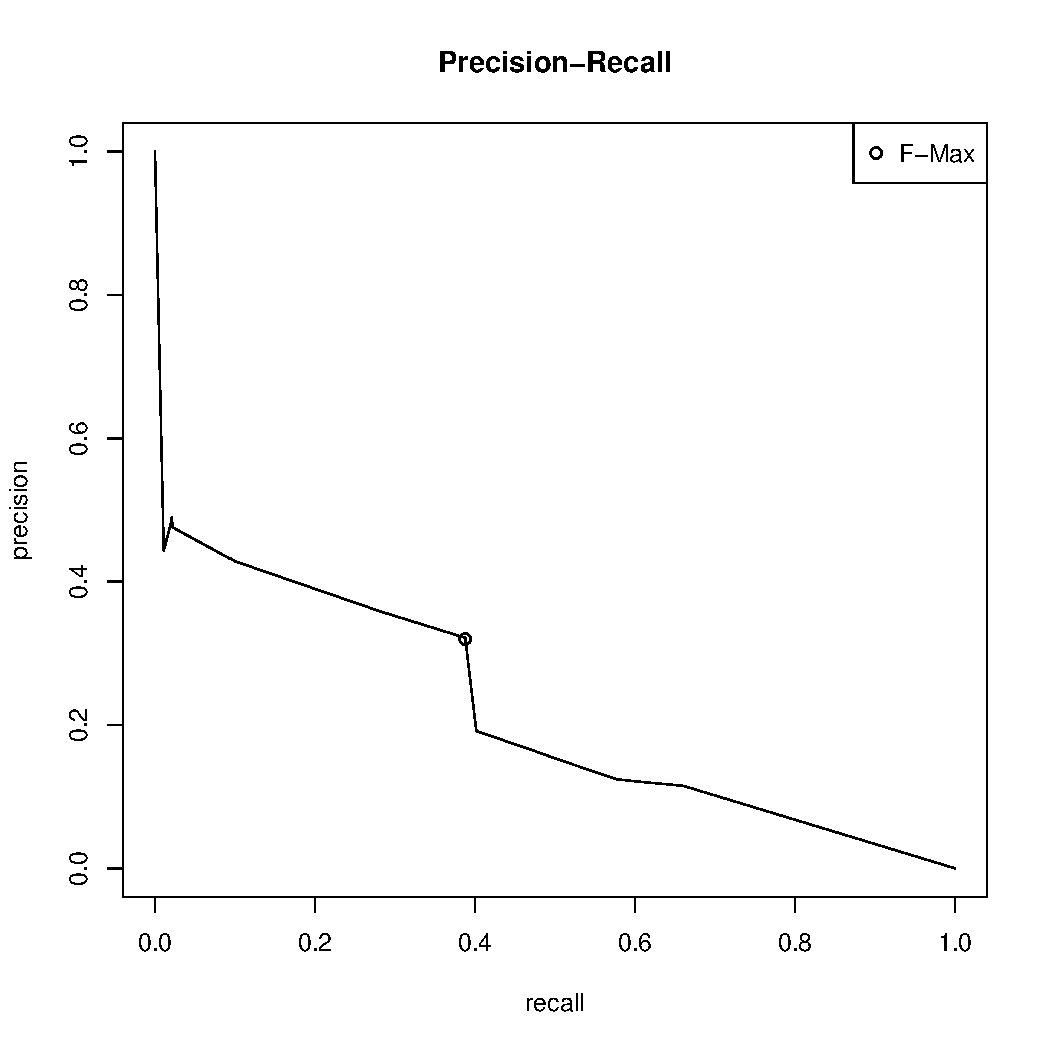
\includegraphics[width=0.5\textwidth]{PreRec_3_folds.pdf}
	\end{center}
	\begin{itemize}
		\item F-measure $0.35\pm0.03$ (at confidence level $0.34$)
		\item Precision $0.32\pm0.04$ (at same confidence level)
		\item Recall  $0.39\pm0.10$ (at same confidence level)
	\end{itemize}		
\end{frame}

%\begin{frame}
%	\frametitle{Results}
%	\begin{center}
%	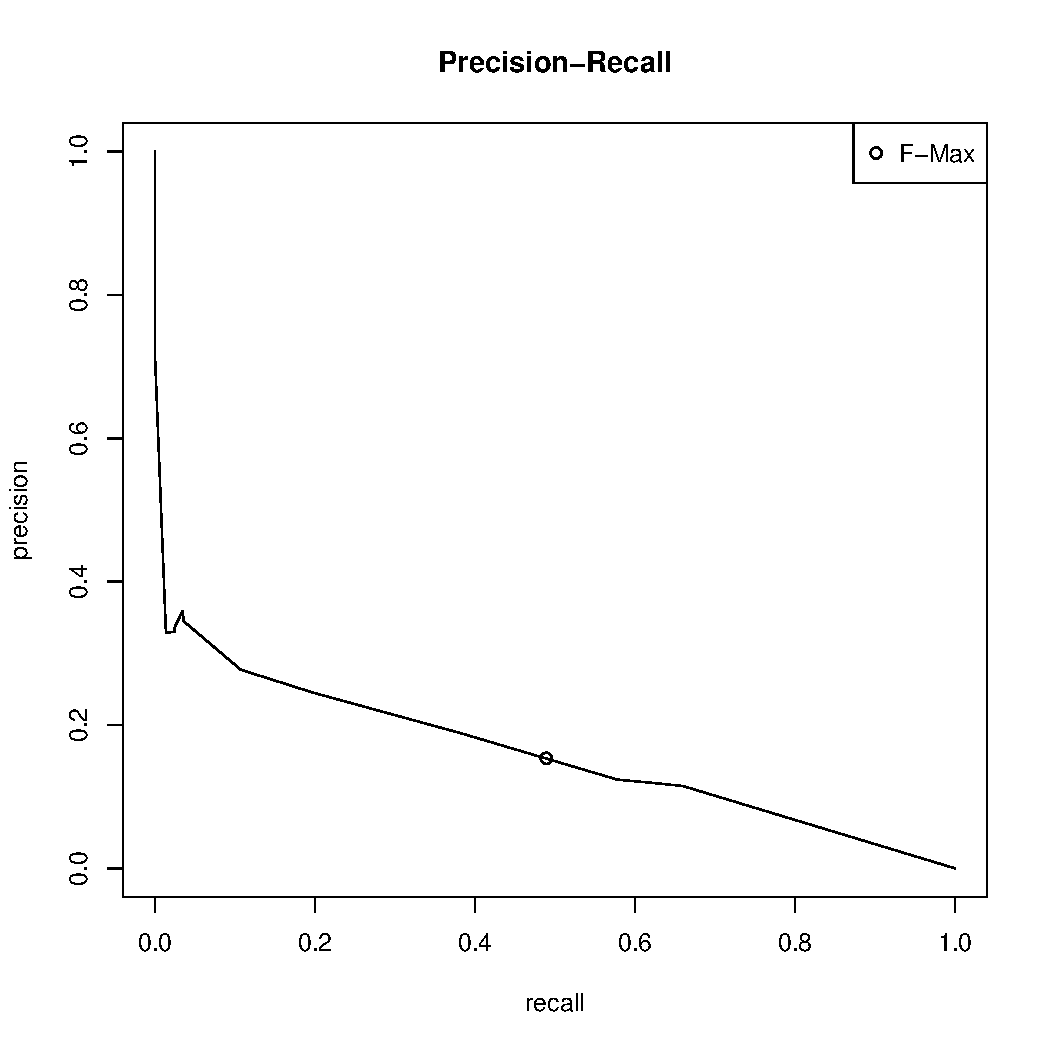
\includegraphics[width=0.5\textwidth]{PreRec_3_avg.pdf}
%	\end{center}
%	\begin{itemize}
%		\item F-measure $0.23\pm0.04$ (at confidence level $0.58$)
%		\item Precision $0.15\pm0.01$ (at same confidence level)
%		\item Recall  $0.49\pm0.02$ (at same confidence level)
%	\end{itemize}		
%\end{frame}

\begin{frame}[fragile]
	\frametitle{HyPnoBrain Online}
\begin{center}
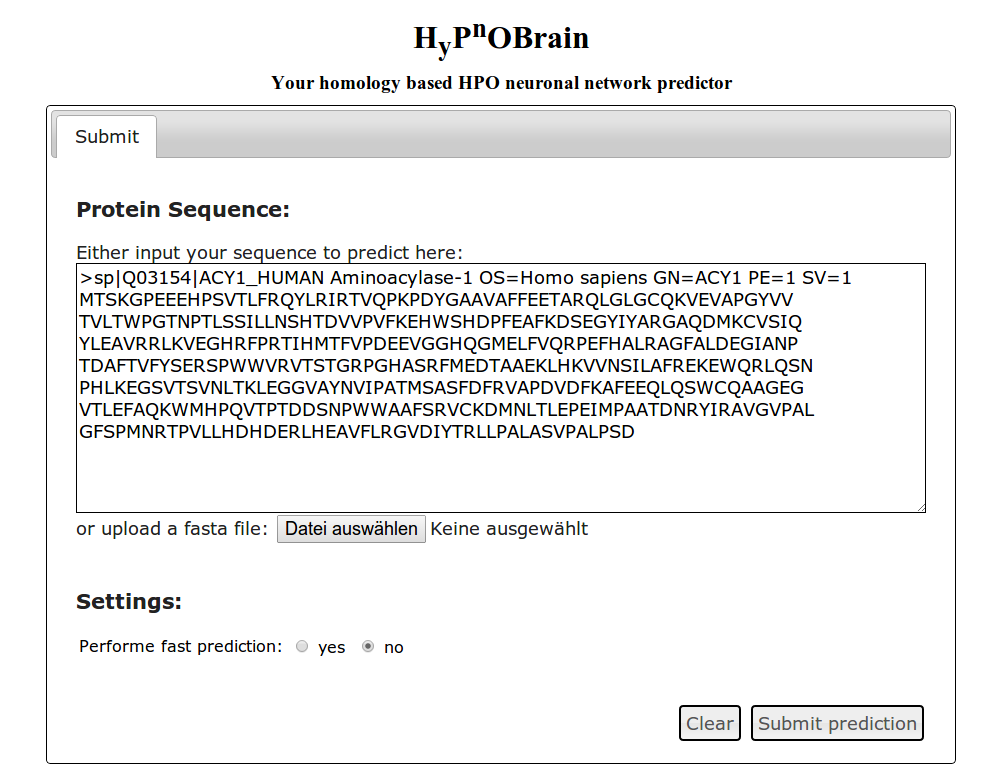
\includegraphics[width=0.7\textwidth]{webinterface.png}
\end{center}

\begin{itemize}
	\item \url{https://dataminer.informatik.tu-muenchen.de/~spoeri/}
	\item file or text field input
	\item option to speed prediction up by restricting hits to 6 best
\end{itemize}

\end{frame}

\begin{frame}
	\frametitle{Productive waste of time aka: Future Improvements}
	\begin{itemize}
		\item Incorporate SVG output of results in webinterface
		\item Feature evaluation and improvement
		\item Investigate effect of homologs in dataset
		\item Different network architectures 
		\item Other machine learning devices
		\item Data mining in other sources
		\item $\dots$
	\end{itemize}		
	
\end{frame}

\end{document}
